\listfiles
\documentclass{article}

\usepackage[pdftex]{graphicx}
\usepackage{amsmath}
\usepackage{amssymb}

\usepackage[a4paper,margin=1in]{geometry}

\newcommand{\half}{\frac{1}{2}}

\title{Loaded Hoop on a conveyer belt}
\date{}

\begin{document}
\maketitle

\section{Preliminary calculations}

\subsection{Acceleration}

Let $v_r$ be the velocity of the load relative to the hoop, $v_x$ be the velocity of the load in the $x$-axis in the lab frame and $v_y$ be the velocity of the load in the $y$-axis in the lab frame. Then

\begin{align*}
v_r = R \dot\theta
\end{align*}

\begin{align*}
v_x &= \dot X + v_r\cos\theta \\
&= \dot X + R \dot\theta\cos\theta \\
v_y &= v_r\sin\theta \\
&= R \dot\theta\sin\theta
\end{align*}

\begin{align*}
a_x &= \dot{v}_x \\
&= \ddot{X} + R\ddot\theta\cos\theta - R\dot\theta^2\sin\theta \\
a_y &= \dot{v}_y \\
&= R\ddot\theta\sin\theta + R\dot\theta^2\cos\theta
\end{align*}

\subsection{Energy}

Let $K_m$ be the kinetic energy of the load, $K_M$ be the kinetic energy of the hoop and $U$ be the potential energy of the load. Then

\begin{align*}
K_m &= \half m (v_x^2 + v_y^2) \\
&= \half m (R \dot\theta\sin\theta)^2 + \half m (\dot X + R\dot\theta\cos\theta)^2 \\
&= \half mR^2\dot\theta^2 + \half m\dot X^2 + mR\dot X\dot\theta\cos\theta \\
\\
K_M &= \half M \dot X^2 + \half M R^2 \dot\theta^2\\
\\
U &= mgR(1 - \cos\theta)
\end{align*}

\begin{align*}
E &= K_m + K_M + U \\
&= \half (M+m) R^2 \dot{\theta}^2 + \half (M+m) \dot{X}^2 + mR\dot\theta \dot X\cos\theta + mgR(1 - \cos\theta)
\end{align*}

\section{Oscillations on a stationary belt}

Let $L$ be the lagrangian $K - U$, ignoring constant terms. Then

\begin{align*}
L &= \half (M+m) R^2 \dot{\theta}^2 + \half (M+m) \dot{X}^2 + mR\dot\theta \dot X\cos\theta + mgR\cos\theta
\end{align*}

\subsection{Period when friction is negligible}

In this case $X$ and $\theta$ are independent variables and we must use the Euler-Lagrange equation on each of them.

\begin{align*}
\frac{\partial L}{\partial \theta} &= -mgR\sin\theta - mR\dot\theta\dot X \sin\theta
\end{align*}

\begin{align*}
\frac{\partial L}{\partial \dot\theta} &= (M+m) R^2 \dot{\theta} + mR \dot X\cos\theta
\end{align*}

\begin{align*}
\frac{d}{dt}\left(\frac{\partial L}{\partial \dot\theta}\right) &= (M+m) R^2 \ddot\theta + mR \ddot X\cos\theta - mR\dot X \dot\theta\sin\theta \\
&= \frac{\partial L}{\partial \theta}
\end{align*}

\begin{align*}
-mgR\sin\theta = (M+m) R^2 \ddot\theta + mR \ddot X\cos\theta \\
mg\sin\theta + (M+m) R \ddot{\theta} + m \ddot X\cos\theta = 0
\end{align*}

We can also obtain this equation by considering $\tau = I\alpha$ about the center of the hoop in the (accelerating) frame of the hoop where $\tau$ is the torque, $I$ the moment of inertia of the system about the center of the hoop and $\alpha = \ddot\theta$ the angular acceleration.

\begin{align*}
I &= (M+m)R^2 \\
\tau &= I \ddot\theta \\
&= - m\ddot X R \sin(\frac{\pi}{2} - \theta) - mgR\sin\theta
\end{align*}

For the $X$-coordinate,

\begin{align*}
\frac{\partial L}{\partial X} &= 0
\end{align*}

\begin{align*}
\frac{\partial L}{\partial \dot X} &= (M+m) \dot{X} + mR\dot\theta\cos\theta
\end{align*}

since $\frac{d}{dt}\left(\frac{\partial L}{\partial \dot X}\right) = \frac{\partial L}{\partial X} = 0, \frac{\partial L}{\partial X}$ is constant. Since $\dot X = \dot\theta = 0$ at the start, $\frac{\partial L}{\partial X} = 0$ always.

\begin{align*}
(M+m) \dot{X} + mR\dot\theta\cos\theta = 0
\end{align*}

We can also obtain this equation by using conservation of horizontal momentum, $M\dot X + mv_x = 0$
\begin{align*}
\dot{X} &= -\frac{m}{M+m} R\dot\theta\cos\theta \\
\ddot{X} &= \frac{m}{M+m} (-R\ddot\theta\cos\theta + R\dot\theta^2\sin\theta)
\end{align*}

combining the two we get

\begin{align*}
mg\sin\theta + (M+m) R \ddot{\theta} + \frac{m^2}{M+m}(R\dot\theta^2\sin\theta\cos\theta - R\ddot\theta\cos^2\theta) = 0
\end{align*}

we now make the approximation that $\theta << 1$, so $\sin\theta = \theta$, $\dot\theta^2 = 0, \cos\theta = 1$

\begin{align*}
mg\theta + (M+m) R \ddot{\theta} - \frac{m^2}{M+m}R\ddot\theta &= 0 \\
\ddot\theta + \frac{m^2 + Mm}{M^2 + 2Mm}\frac{g}{R}\theta &= 0 \\
\omega^2 = \frac{m^2 + Mm}{M^2 + 2Mm}\frac{g}{R}
\end{align*}

where $\omega$ is the angular velocity. Hence the period $T = \frac{2\pi}{\omega} = 2\pi \sqrt{\frac{M^2 + 2Mm}{m^2 + Mm}\frac{R}{g}}$

\subsection{Period when the hoop does not slip}

The non-slip condition occurs when the velocity of the contact point between the hoop and the floor is $0$.

\begin{align*}
\dot X + R\dot\theta = 0
\end{align*}

We can simplify the Lagrangian with this

\begin{align*}
L = (M+m)R^2\dot\theta^2 - mR^2\dot\theta^2\cos\theta + mgR\cos\theta
\end{align*}

notice that horizontal momentum is not conserved since there is an external frictional force which has a horizontal component. However since this is static friction which does no work, energy is conserved and the ELE can still be used.

\begin{align*}
\frac{\partial L}{\partial \dot\theta} = 2(M+m)R^2\dot\theta\ - 2mR^2\dot\theta\cos\theta
\end{align*}

\begin{align*}
\frac{d}{dt} \frac{\partial L}{\partial \dot\theta} = 2(M+m)R^2\ddot\theta - 2mR^2\ddot\theta\cos\theta + 2mR^2\dot\theta^2\sin\theta
\end{align*}

\begin{align*}
\frac{\partial L}{\partial \theta} = m  R^2\dot\theta^2\sin\theta - mgR\sin\theta
\end{align*}

\begin{align*}
2MR\ddot\theta + mg\theta &= 0 \\
\ddot\theta + \frac{m}{2M}\frac{g}{R}\theta &= 0
\end{align*}

Alternatively, we can also introduce $f$ as the friction force.

\begin{align*}
f &= M\ddot{X} + ma_x \\
&=M\ddot{X} + m\ddot{X} + mR\ddot\theta\cos\theta - mR\ddot\theta^2\sin\theta \\
&\approx M\ddot{X}
\end{align*}

this makes sense as for small $\theta$ the load is close to the point of contact between the ground and the hoop, which is almost stationary in the non-slip condition. Using $\tau = I\ddot\theta$ again

\begin{align*}
(M+m)R^2\ddot\theta &= fR - m\ddot{X}\cos\theta R - mgR\sin\theta \\
(M+m)R\ddot\theta &= -MR\ddot\theta + mR\ddot\theta - mg\sin\theta \\
\end{align*}

\begin{align*}
2MR\ddot\theta + mg\sin\theta = 0
\end{align*}

hence,

\begin{align*}
\omega^2 = \frac{m}{2M}\frac{g}{R}
\end{align*}

and the period $T = 2\pi\sqrt{\frac{2M}{m}\frac{R}{g}}$

\section{Stable Angular Orientations on an Accelerating Conveyer Belt}

Let $a = \ddot{X}$ be the (constant) acceleration of the hoop and load.

In the frame of the accelerating system, we can balance torques about the center of the hoop:

\begin{align*}
f = mg\sin\theta + ma\cos\theta
\end{align*}

Balancing forces

\begin{align*}
f = (M+m)a
\end{align*}

equating the two

\begin{align*}
(M+m)a = mg\sin\theta + ma\cos\theta
\end{align*}

now choose $k$ and $\phi$ such that $k\sin\phi = a$ and $k\cos\phi = g$; $k$ and $\phi$ will obviously always exist because we have not reduced the number of degrees of freedom (2) and $k$ is unbounded. Then

\begin{align*}
\phi &= \tan^{-1}{\frac{a}{g}} \\
k &= \sqrt{a^2 + g^2}
\end{align*}

Now

\begin{align*}
(M+m)a &= mk\cos\phi\sin\theta + mk\sin\phi\cos\theta \\
&= mk\sin(\phi + \theta) \\
\frac{M+m}{m}\frac{a}{k} &= \sin(\phi + \theta)
\end{align*}

\begin{align*}
\phi + \theta &= \sin^{-1}{\frac{M+m}{m}\frac{a}{k}} \\
\theta &= \sin^{-1}{\frac{M+m}{m}\frac{a}{k}} - \phi \\
&= \sin^{-1}{\frac{M+m}{m}\frac{a}{\sqrt{a^2 + g^2}}} - \tan^{-1}{\frac{a}{g}}
\end{align*}

or, in terms of $\gamma = \frac{m}{M}$,

\begin{align*}
\theta &= \sin^{-1}((1 + \frac{1}{\gamma}) \frac{a}{\sqrt{a^2 + g^2}}) - \tan^{-1}{\frac{a}{g}}
\end{align*}

\subsection{$\mu_s = 1.0$}

There are two cases we have to consider; either the friction is kinetic or static in nature. For static friction, 

\begin{align*}
a = K = \sqrt{3}g
\end{align*}

\begin{align*}
f &= (M+m)a \\
&= (M+m)\sqrt{3}g
\end{align*}

Let $N$ be the normal frictional force. Balancing forces in the vertical direction,

\begin{align*}
N &= (M+m)g
\end{align*}

unfortunately, $f > \mu_sN$. Hence, the friction must be kinetic in nature.

\begin{align*}
f &= \mu_kN \\
&= \frac{\sqrt 3}{3}(M+m)g
\end{align*}

and since $f = (M+m)a$,

\begin{align*}
a &= \frac{\sqrt 3}{3}g
\end{align*}

and

\begin{align*}
\frac{a}{\sqrt{a^2 + g^2}} = \half
\end{align*}

and since $\frac{a}{g} = \frac{\sqrt 3}{3}$ and $\tan^{-1} \frac{\sqrt 3}{3} = \frac{\pi}{6}$, hence

\begin{align*}
\alpha_1 &= \sin^{-1}((1 + (\frac{m}{M})^{-1}) \half) - \frac{\pi}{6}
\end{align*}

\subsection{$\mu_s = 2.0$}

In this case, for static friction, the working is the same; we still have

\begin{align*}
f &= (M+m)\sqrt{3}g \\
N &= (M+m)g
\end{align*}

but now $f < \mu_s N$ because $\sqrt 3 < 2$. Hence $a = \sqrt{3}g$ and

\begin{align*}
\frac{a}{\sqrt{a^2 + g^2}} = \frac{\sqrt{3}}{2}
\end{align*}

and since $\frac{a}{g} = \sqrt{3}$ and $\tan^{-1} \sqrt 3 = \frac{\pi}{3}$, hence

\begin{align*}
\alpha_2 &= \sin^{-1}((1 + (\frac{m}{M})^{-1}) \frac{\sqrt{3}}{2}) - \frac{\pi}{3}
\end{align*}

\section{Oscillation, Rotation, and Sliding on an Accelerating Conveyor Belt}

\subsection{Type A motion}

Let $x$ be the position of the center of the hoop relative to the point on the belt it was first placed on in a frame of reference moving at acceleration $K$ (thus $X = \half Kt^2 + x$). Then in this frame, the conveyor belt is stationary; hence friction does no work. The fictitious force does work $W_{fic}$on the system

\begin{align*}
W_{fic} &= MKx + mK(x + R\sin\theta)
\end{align*}

by the work-energy theorem,

\begin{align*}
MKx + mK(x + R\sin\theta) + \half (M+m) R^2 \dot{\theta}^2 + \half (M+m) \dot{x}^2 + mR\dot\theta \dot x\cos\theta + mgR(1 - \cos\theta) = 0
\end{align*}

since it is constant and $x, \dot{x}, \theta, \dot{\theta}$ were all 0 initially. The non-slip condition is that

\begin{align*}
x + R\theta = 0
\end{align*}

simplifying,

\begin{align*}
-MKR\theta + mKR(\sin\theta - \theta) + (M+m) R^2 \dot{\theta}^2 - mR^2\dot\theta^2\cos\theta + mgR(1 - \cos\theta) = 0
\end{align*}

with $M=m$,

\begin{align*}
K(\sin\theta - 2\theta) + R \dot{\theta}^2 (2 - \cos\theta) + g(1 - \cos\theta) = 0
\end{align*}

\begin{align*}
R \dot{\theta}^2 (2 - \cos\theta) &= K(2\theta - \sin\theta)+ g(\cos\theta - 1) \\
R \dot{\theta}^2 &= \frac{K(2\theta - \sin\theta)+ g(\cos\theta - 1)}{(2 - \cos\theta)} \\
\half MR^2 \dot{\theta}^2 &= \half MR \frac{K(2\theta - \sin\theta)+ g(\cos\theta - 1)}{(2 - \cos\theta)}
\end{align*}

This means that the system is equivalent to a point of mass $M$ in a one-dimensional potential $V(\theta) \sim \frac{K(2\theta - \sin\theta)+ g(\cos\theta - 1)}{(\cos\theta - 2)}$. Assuming that $V < 0$ when $0 < \theta < \beta$, when $\theta = \theta_{maximum}$, $\dot\theta = 0$ because otherwise we can increase $\theta$ by $d\theta$ by increasing or decreasing $t$ by $dt$. Another way to see this is that in the equivalent system, $V = 0$ when $\theta = 0$; hence $\theta$ will oscillate between two roots of $V$. Hence

\begin{align*}
K(\sin\beta - 2\beta) + g(1 - \cos\beta) = 0
\end{align*}

\begin{align*}
\frac{K}{g} &= \frac{1 - \cos\beta}{2\beta - \sin\beta} \\
&= 0.244837712
\end{align*}

with $\beta = \frac{\pi}{6}$. Now we plot $V(\theta)$ up to multiplicative constants for $\frac{K}{g} = 0.245$

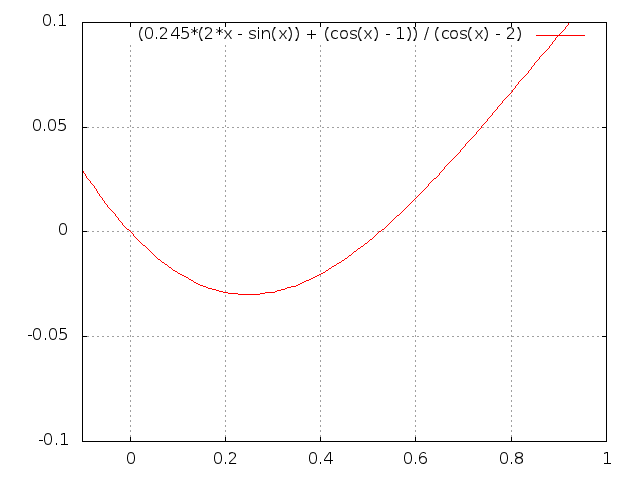
\includegraphics[width=\textwidth]{4A1.png}
We see that the particle will exhibit Type A motion, oscillating between the two roots of $V(\theta)$

\subsection{Type B motion}

If we try $\beta = \pi$,

\begin{align*}
\frac{K}{g} &= \frac{1 - \cos\beta}{2\beta - \sin\beta} \\
&= 0.318
\end{align*}

Now we plot $V(\theta)$ up to multiplicative constants for $\frac{K}{g} = 0.318$. 

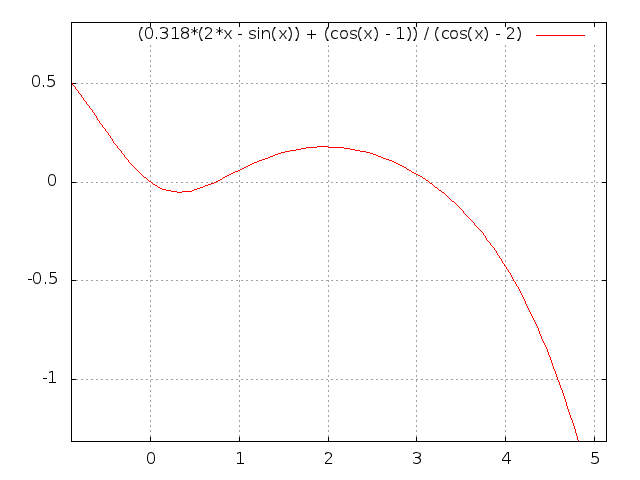
\includegraphics[width=\textwidth]{fail.png}

Although $V = 0$ at $\theta = \pi$, there is a positive-energy barrier (hump) where $V > 0$ as $0 < \theta < \pi$, preventing the particle from reaching $\theta = \pi$.

Hence the condition that $\dot\theta = 0$ is insufficient; we must also make sure that $V < 0$ as $0 < \theta < \pi$. Since $\cos\theta - 2 < 0$, this is equivalent to making $Z < 0$ where

\begin{align*}
Z = -K(2\theta - \sin\theta) - g(\cos\theta - 1)
\end{align*}

the local maximum occurs when

\begin{align*}
\frac{dZ}{d\theta} &= 0 \\
K(2 - \cos\theta) - g\sin\theta &= 0 \\
2K - (K\cos\theta + g\sin\theta) &= 0 \\
2K - \sqrt{K^2 + g^2}\sin(\theta + \tan^{-1}\frac{K}{g}) &= 0 \\
\sin(\theta + \tan^{-1}\frac{K}{g}) &= \frac{2K}{\sqrt{K^2 + g^2}}
\end{align*}

Let $\theta_{Zmax}$ be the positive $\theta$ such that $Z$ is maximized. Then $\theta_{Zmax}$ is the second root because as seen from the graph, the first root corresponds to a local minimum while the second root corresponds to a local maximum. 

\begin{align*}
\theta_{Zmax} &= \pi - \sin^{-1}(\frac{2K}{\sqrt{K^2 + g^2}}) - \tan^{-1}\frac{K}{g}\\
\end{align*}

We want to find $\frac{K}{g}$ such that $Z(\theta_{Zmax}) < 0$, so (substituting the expression for $\theta_{Zmax}$ into $Z(\theta)$) we must find the root of

\begin{align*}
-1 - \cos\left(\sin^{-1}\frac{2\gamma}{(\sqrt{1+\gamma^2})} + \tan^{-1}\gamma\right) + \gamma\left(2\pi - 2\sin^{-1}\frac{2\gamma}{\sqrt{1+\gamma^2}} - 2\tan^{-1}\gamma - \sin(\sin^{-1}\frac{2\gamma}{\sqrt{1+\gamma^2}} + \tan^{-1}\gamma)\right)
\end{align*}

with $\gamma = \frac{K}{g}$. Solving numerically, $\gamma = 0.4687 = 0.47$ (2 s.f.)

We now plot $V(\theta)$ up to multiplicative constants for two values of $\frac{K}{g} > \gamma$

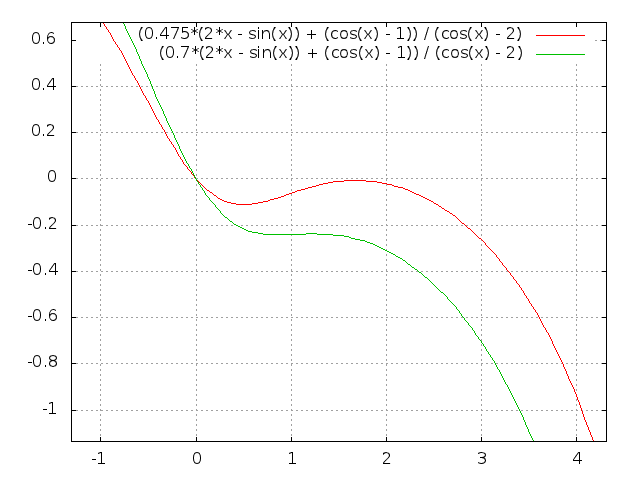
\includegraphics[width=\textwidth]{4A2.png}

Indeed, there are no longer any barriers.

\subsection{Sliding motion}

By force analysis in the horizontal direction,

\begin{align*}
f - (M+m)K &= M\ddot{x} + ma_x \\
&= - MR\ddot\theta - mR\ddot\theta(1 - \cos\theta) - mR\dot\theta^2\sin\theta
\end{align*}

\begin{align*}
f = (M+m)K - MR\ddot\theta - mR\ddot\theta(1 - \cos\theta) - mR\dot\theta^2\sin\theta
\end{align*}

with $M = m$,

\begin{align*}
f = 2MK - MR\ddot\theta(2 - \cos\theta) - MR\dot\theta^2\sin\theta
\end{align*}

Recall that 

\begin{align*}
\half MR^2 \dot{\theta}^2 &= \half MR \frac{K(2\theta - \sin\theta)+ g(\cos\theta - 1)}{(2 - \cos\theta)}
\end{align*}

differentiating with respect to $\theta$,

\begin{align*}
MR^2 \dot\theta \frac{d\dot\theta}{d\theta} &= \half MR \left(\frac{K(2\theta - \sin\theta)+ g(\cos\theta - 1)}{(2 - \cos\theta)}\right)'
\end{align*}

but since

\begin{align*}
\dot\theta \frac{d\dot\theta}{d\theta} &= \frac{d\theta}{dt} \frac{d\dot\theta}{d\theta} \\
&= \ddot\theta
\end{align*}

hence

\begin{align*}
R \ddot\theta &= \half \left(\frac{K(2\theta - \sin\theta)+ g(\cos\theta - 1)}{(2 - \cos\theta)}\right)'
\end{align*}

also

\begin{align*}
R \dot\theta^2 &= \frac{K(2\theta - \sin\theta)+ g(\cos\theta - 1)}{(2 - \cos\theta)}
\end{align*}

substituting,

\begin{align*}
f = 2MK - \half M \left(\frac{K(2\theta - \sin\theta)+ g(\cos\theta - 1)}{(2 - \cos\theta)}\right)'(2 - \cos\theta) - M\frac{K(2\theta - \sin\theta)+ g(\cos\theta - 1)}{(2 - \cos\theta)}\sin\theta
\end{align*}

by a similar procedure but analyzing forces in the vertical direction,

\begin{align*}
N = 2Mg + \half M\left(\frac{K(2\theta - \sin\theta)+ g(\cos\theta - 1)}{(2 - \cos\theta)}\right)'\sin\theta + M\frac{K(2\theta - \sin\theta)+ g(\cos\theta - 1)}{(2 - \cos\theta)}\cos\theta
\end{align*}

Let $\mu_e = \frac{f}{N}$. $\mu_{s,0}$ will be the maximum value of $\mu_e$ for $0 \le \theta \le \frac{\pi}{6}$ because if $\mu_s$ is less than that, then at some point in the system's motion (ie, for some $\theta$) we will have $f > \mu_s N$.

\begin{align*}
\mu_{e} = \frac{2K - \half \left(\frac{K(2\theta - \sin\theta)+ g(\cos\theta - 1)}{(2 - \cos\theta)}\right)'(2 - \cos\theta) - \frac{K(2\theta - \sin\theta)+ g(\cos\theta - 1)}{(2 - \cos\theta)}\sin\theta}{2g + \half \left(\frac{K(2\theta - \sin\theta)+ g(\cos\theta - 1)}{(2 - \cos\theta)}\right)'\sin\theta + \frac{K(2\theta - \sin\theta)+ g(\cos\theta - 1)}{(2 - \cos\theta)}\cos\theta}
\end{align*}

\begin{align*}
\left(\frac{K(2\theta - \sin\theta)+ g(\cos\theta - 1)}{(2 - \cos\theta)}\right)' = \frac{5K - g\sin\theta - 4K\cos\theta - 2K\theta\sin\theta}{(2-\cos\theta)^2}
\end{align*}

\begin{align*}
\mu_{e} = \frac{2K - \frac{5K - g\sin\theta - 4K\cos\theta - 2K\theta\sin\theta}{4-2\cos\theta} - \frac{K(2\theta - \sin\theta)+ g(\cos\theta - 1)}{(2 - \cos\theta)}\sin\theta}{2g + \half  \frac{5K - g\sin\theta - 4K\cos\theta - 2K\theta\sin\theta}{(2-\cos\theta)^2}\sin\theta + \frac{K(2\theta - \sin\theta)+ g(\cos\theta - 1)}{(2 - \cos\theta)}\cos\theta}
\end{align*}

plotting this

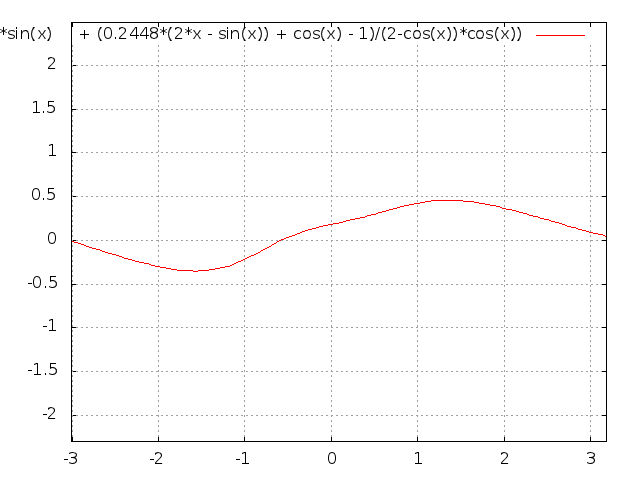
\includegraphics[width=\textwidth]{mu.png}

we see that the maximum value of $\mu_e$ for $0 \le \theta \le \frac{\pi}{6}$ is at $\theta = \frac{\pi}{6}$. Plugging in, $\mu_{s,0} = 0.307955 = 0.31$ (2 s.f.)


\end{document}
